\documentclass[output=paper]{langsci/langscibook} 
\ChapterDOI{10.5281/zenodo.5040306}

\author{Sampriti Mahanty\affiliation{University of Manchester} and
Frank Boons\affiliation{University of Manchester} and
Julia Handl\affiliation{University of Manchester} and
Riza Batista-Navarro\affiliation{University of Manchester}
}

\title[Computation of semantic change in scientific concepts]
      {Computation of semantic change in scientific concepts: Case study of ``circular economy''}


\abstract{In this chapter we aim to investigate semantic change in a scientific concept underpinned by the evolutionary framework of scientific knowledge production. The aim of this article is threefold. First is to distinguish semantic change computation in scientific concepts from that in core vocabulary and slang. Second is a multi-step analysis combining topic modelling, co-occurence networks and word embeddings, along with a control condition setup thereby presenting a pipeline to compute semantic change in a scientific concept. Third is an analysis of a popular concept in sustainability studies, i.e., ``circular economy'', seeking to advance research on this concept. In order to achieve our objectives, we use topic modelling to detect the point of change in a literature corpus and then we apply two approaches for detecting semantic change: co-occurence networks and word embeddings. Furthermore, we compare the concept with other related concepts in the same semantic field and use word embeddings to detect if the concept has undergone any changes relative to other concepts.}



\begin{document}
\SetupAffiliations{mark style=none}
\maketitle

\section{Introduction}
Scientists contribute to the process of scientific knowledge production acting as the \textit{central subjects} in this process. They are the entities who read the literature, perform experiments, publish the results and pass on knowledge. Textbooks and journal articles serve as \textit{vehicles} in this process \citep{hull1988science}. Philosophers of science have conceptualised this process of scientific knowledge production to be \textit{evolutionary} \citep{toulmin1972human,hull1988science}, drawing analogies with biological evolution where concepts are linguistic labels given to abstract ideas \citep{fodor1975language,pinker1994language} which are framed, selected, re-conceptualised, discarded leading to a continuous evolution of the language used by researchers \citep{boons2017industrial}. In order to define these concepts, members of the scientific community build upon the same language (i.e., lexicon-kind terms) at the very least. Language, thus, becomes a crucial indicator to assess the shift or development in ideas \citep{kuhn1990road}. Whilst philosophers of science have given much attention to scientific knowledge production in evolutionary terms, we intend to focus on this work from a computational perspective to understand how we can use computational methods to detect evolution in scientific knowledge production.

In the past decade an emerging research topic in the field of computational linguistics has been on the topic of semantic change computation \citep{tang2018state}. Semantic change refers to any change in the word meaning over a period of time.  Semantic change in words can sometimes happen to the extent that the modern meaning is radically different. In some cases, the semantic change that words undergo happens by means of acquiring additional meanings, rather than original meanings becoming outdated or being replaced. We find useful the definition put forward by \citet{bloomfield-1933}, where lexical semantic shifts or semantic change is defined as ``innovations which change the lexical meaning rather than the grammatical function of a form''. In the process of scientific knowledge production, any change in science is termed as evolution of science, thus taking \textit{change} and \textit{evolution} to be synonymous \citep{wuketits1984evolutionary,bradie1986assessing}. Drawing from this we set out to understand the evolution of concepts in the scientific literature through the lens of semantic change. Thus, we propose that when there is an evolution in concepts over time, it can be detected through computation of semantic change. From an empirical perspective, a key assumption is that changes in a concept's collocational patterns reflect changes in concept meaning, thus providing a usage-based account of semantics.

We begin by analysing the related work and positioning of the research in Section~\ref{ch03:relwork}. In Section~\ref{ch03:casestudy} we present the case study for this research. In Section~\ref{ch03:method} we discuss the methodology in detail and present the results based on our case study in Section~\ref{ch03:experiments}. Finally, we present the discussion and conclusion in Section~\ref{ch03:discussion}.

\section{Analysis of related work and positioning of the research}\label{ch03:relwork}
There are a number of studies which have harvested the availability of huge diachronic language data to advance the research on semantic change computation \citep{sagi-etal-2009-semantic, michel2011quantitative, rohrdantz2011towards, jatowt:2014:fas:2740769.2740809, mitra2015automatic, frermann-lapata-2016-bayesian, hamilton-etal-2016-diachronic, tang2016,dubossarsky-etal-2017-outta}. From a computational perspective, semantic change has been approached from two aspects: word-level semantic change and concept-level semantic change \citep{tahmasebi2018survey}. There have been a number of studies which have focused on concept-level semantic change providing valuable insights such as the idea of concept through time (CTT, \citealt{wevers2015concepts}), parallelogram model of analogy \citep{orlikowski-etal-2018-learning} and tracing concept vocabularies through a time-stamped corpus \citep{kenter2015ad, recchia2016tracing}. However, there have been different ways in which the label of a concept has been approached in different studies. Since different domains have different interpretations of what a concept means, it should also be appreciated that any definition of a concept has a sense of arbitrariness and it is therefore desirable to study concepts with as much flexibility as possible \citep{fokkens2016semantics}. For instance, in studies by \citet{kenter2015ad} and \citet{orlikowski-etal-2018-learning}, there are concept terms which make up the conceptual core (core concept terms) from the rest of the vocabulary (characterising concept terms), thus distinguishing between the core and the margin of concepts. For example, for the concept of ``economic efficiency'', core terms might be \emph{efficiency} and \emph{efficient}, while characterising terms might be \emph{robotisation}, \emph{automatisation} or \emph{labor productivity}. In other studies such as \citet{wang2011concept}, concepts not only exist in the textual information in the documents, but also refer to the quantity that a learning model is trying to predict, i.e., the variables. However, the understanding of \emph{concept} that we use in this paper is based on some interpretations of the classical theory of concepts which treat concepts as a one-to-one correspondence with word senses \citep{sep-concepts}. While there are a number of schools of thought pertaining to the definition of a concept, the understanding that we adopt in this article allows us to assess the evolution of a particular concept that is used in scientific literature. Thus, going by the parsimonious understanding of a concept in our study, if we were to investigate the evolution of the ``economic efficiency'' concept in scientific literature, we would focus on it verbatim and possibly other forms with affixes, suffixes or short forms such as \emph{economically efficient}, \emph{eco-efficiency}, etc.

Hence, our computational approach is based on what has been called word-level semantic change in previous research. However, there are certain aspects which make our study distinct from previous research and bring about the novelty. The first aspect is concerned with the nature of the data and the second aspect is concerned with the rate of change.

\begin{description}
\item[Nature of data used:] Previous studies of word-level semantic change detection are mostly based on data sources such as the Google Books Ngram corpus which is the largest text corpus used in semantic studies \citep{michel2011quantitative,gulordava-baroni-2011-distributional,hamilton-etal-2016-diachronic,jatowt:2014:fas:2740769.2740809,xu15,dubossarsky-etal-2017-outta}, the Corpus of Historical American English (COHA) \citep{hamilton-etal-2016-diachronic,neuman2017information} and the Helsinki corpus of English texts \citep{sagi-etal-2009-semantic}. Apart from the use of such text corpora, Twitter \citep{mitra2015automatic} has also been used. For the purpose of this work, our interest is in concepts used in scientific literature and we find that work on semantic change based on scientific literature is limited. \citet{chen2018semantic} studied semantic changes in a scientific domain by analysing the same words which have different meanings in different domains. \citet{rudolphb18-dynamicembforlangevo} developed dynamic word embeddings using data from Association for Computing Machinery (ACM) abstracts and machine learning papers on the preprint database arXiv. However, most studies which use academic journal articles and abstracts as a corpus are in the biomedical domain where the classic research problem focuses on semantic relatedness and similarity between biomedical terms \citep{zhu2017semantic}. A recent development on computational analysis of scientific literature has been the release of SciBERT, a new resource based on contextual embeddings demonstrated to improve performance on a range of natural language processing (NLP) tasks in the scientific domain. SciBERT is a pre-trained language model based on BERT but trained on a large corpus of scientific text \citep{beltagy2019scibert}. In our study, we do not make use of SciBERT since: (1) we do not have access to a large enough ``circular economy'' corpus for training our own model, and (2) their publicly available pre-trained model was trained on a corpus where 18\% of the papers were drawn from the computer science domain and 82\% from the biomedical domain. Due to its narrow focus in terms of domains it is not applicable in our context. Thus, to the best of our knowledge there has been limited attention on semantic change drawn from scientific literature barring a few exceptions like the study by \citet{dridi2019leap2trend} which provides interesting insights on how to use temporal word embeddings to detect emerging scientific trends, although they do not specifically focus on semantic change. Furthermore, delving into the nature of the data, \citet{MelvinWeversandMarijnKoolenKoolen2020} put forward certain considerations to reflect on before training a word embedding model for computation of semantic change, i.e., (1) large enough data size spanning long time periods, (2) identification of optical character recognition (OCR) errors and spelling variations in the data, and (3) cultural and political bias in the data. These factors could affect the quality of the model being trained. However, we question if these hold true when using scientific literature as the corpus. For instance, for scientific concepts, the time period might not need to be so long as there is evidence of structural changes even within short time periods \citep{mahanty2019studying}, which we believe can be detected through semantic change computation. Due to shorter time periods, the data that is available to study semantic change of concepts in scientific literature is often much smaller compared to studies using newspaper articles, Twitter data, movie reviews and books. Scientific text is more likely to be devoid of noise like OCR errors and spelling variations. Ideally, scientific literature is also devoid of any cultural and political bias since most journals have a criteria of using inclusive language in articles. Thus, the data drawn from scientific literature is of much better quality, therefore increasing the chances of obtaining a better trained model.

\item[Rate and nature of semantic change:] There are systemic irregularities in the rate of semantic change of words wherein the rate of change of some words is higher than that of others \citep{hamilton-etal-2016-diachronic}. Studies have established that the distributional properties of words implicate semantic change by showing that verbs change at a faster rate than nouns \citep{dubossarsky2016verbs}. Another study by \citet{greenhill2017evolutionary} is along the same line of thought and it again provides evidence on different rates of change in different aspects of language. They show that, in general, grammatical features tend to change faster and have higher amounts of conflicting signals than basic vocabulary, suggesting that subsystems of language show differing patterns of dynamics. When extending this to scientific concepts, we hypothesise that there is a difference in the rate of change between scientific concepts, core vocabulary and slang. While core vocabulary has been found to be more stable \citep{bengtson2011basque}, slang words are ephemeral \citep{wang2020analysis}. Meanwhile, scientific concepts often undergo changes such as reconceptualisation, recombination and relabelling in the process of evolution \citep{bradie1986assessing}, and are therefore borrowed, adapted or inflated. Thus, a blanket case of semantic change might not fit for scientific concepts.
\end{description}

This chapter focusses on the development of a computational pipeline for assessing conceptual evolution in the process of scientific knowledge production based on journal articles and abstracts. From a conceptual evolution perspective there are two aspects that can be investigated, i.e., firstly the evolution of a scientific concept exclusively and then the evolution of the concept with respect to other concepts in the same ``semantic field''. Since we understand evolution of scientific concepts by the evolution of language used by scientists, we address the first strand of our work by analysing the change in a concept's associated vocabulary. Meanwhile, for the latter strand of this work, we will investigate what is called a ``semantic field'', which is defined as a set of words which cover a particular semantic domain and bear structured relations with one another \citep{jurasky2000speech}. 
Semantic fields can be studied diachronically or synchronously. The former focusses on  the origin and transformation of specific concepts while the latter deals with concepts appearing and their connection with other concepts. Thus, the understanding of a semantic field allows a better understanding of the meaning and the context of a concept with respect to other concepts. Our second goal will be to develop a computational pipeline to understand the evolution of a concept with respect to other concepts in the semantic field. In our previous work, we assessed the evolution of a concept using topic modelling \citep{mahanty2019studying}.  While that work enabled us to computationally detect conceptual evolution to some extent, we did not uncover the extent of change or evolution, nor determined if the change is statistically significant. These are now addressed in the work described in this chapter. Furthermore, building upon our previous work, we perform a comparison of a number of concepts within the same semantic field thereby tracing the shift in their contexts. 

Our contribution in this article are the following:

\begin{enumerate}[label=\alph*.]
\item We establish a case for semantic change in scientific concepts and its difference compared to core vocabulary and slang.
\item From a methodological perspective, we present a pipeline based on multi-angle analysis combining different methods along with a control condition setup for computation of semantic change. This can be broadly applied across disciplines to analyse a vast and expanding literature on any concept.
\item From an application perspective, this study provides insights on a very popular concept in sustainability studies.
\end{enumerate}

\section{Case study: The concept of ``circular economy''}\label{ch03:casestudy}
In the sustainability debate, the concept of ``circular economy'' (CE) has received immense traction amidst scholars, practitioners and policymakers in the recent years. CE refers to a system of provision in which resources are circulated between production and consumption rather than linearly transformed from production to consumption to waste. An example of CE application would be ``Garment Collecting Program'' of H\&M, which was the result of a partnership between H\&M and I:CO. This project aims at collecting and propose to their customers the used clothes at the firm's stores in three ways: ``(i) rewear, i.e. clothing that can be worn again will be sold as second hand clothes; (ii) reuse, i.e. old clothes and textiles will be turned into other products, such as cleaning cloths; (iii) recycle, i.e. everything else is turned into textile fibers, or other use such as insulation'' \citep{urbinati2017towards}.

While the CE term was coined by \citet{pearce1990economics} it mostly underwent a dormant phase until early 2000s apart from a few mentions, for example, \citet{cooper1994beyond, cooper1999creating}. But from the early 2000s it has received immense attention in the academic discourse with over 1000 academic articles published in a single year. It became a popular policy agenda across European countries, China and Latin America. Another interesting aspect of CE is its relation to other concepts. The concept of CE is often studied in relation to other concepts such as ``bio-economy'', ``green-economy'' \citep{d2017green}, ``cradle to cradle'', ``industrial ecology'', ``closed loop supply chains'', ``regenerative design'', ``blue economy'', ``industrial symbiosis'', ``reverse logistics'', ``performance economy'', ``natural capitalism'', and ``biomimicry'' \citep{geisendorf2018circular}. Some of these concepts are termed as the antecedents to the CE concept or CE schools of thought \citep{homrich2018circular}. While we assess the changes in the CE concept, it is also of interest to understand how it is evolving in relation to other concepts. It might also provide further evidence of evolution in the concept of CE, if there is any.

Thus, we use the concept of ``circular economy'' as a case study to fulfil two of our goals i.e.,

\begin{enumerate}[label=\alph*.]
\item study the evolution of a concept exclusively
\item study the evolution of a concept in relation to other concepts in a semantic field.
\end{enumerate}

We aim to uncover the conceptual evolution of the concept ``circular economy'' in academic literature through computational analysis of semantic change. We use academic articles published on CE from 2005 to 2019. 

\section{Methodology}\label{ch03:method}
In this section we discuss our methodology in detail. Figure~\ref{ch03:fig1} is a brief representation of the methodology.

\begin{figure}
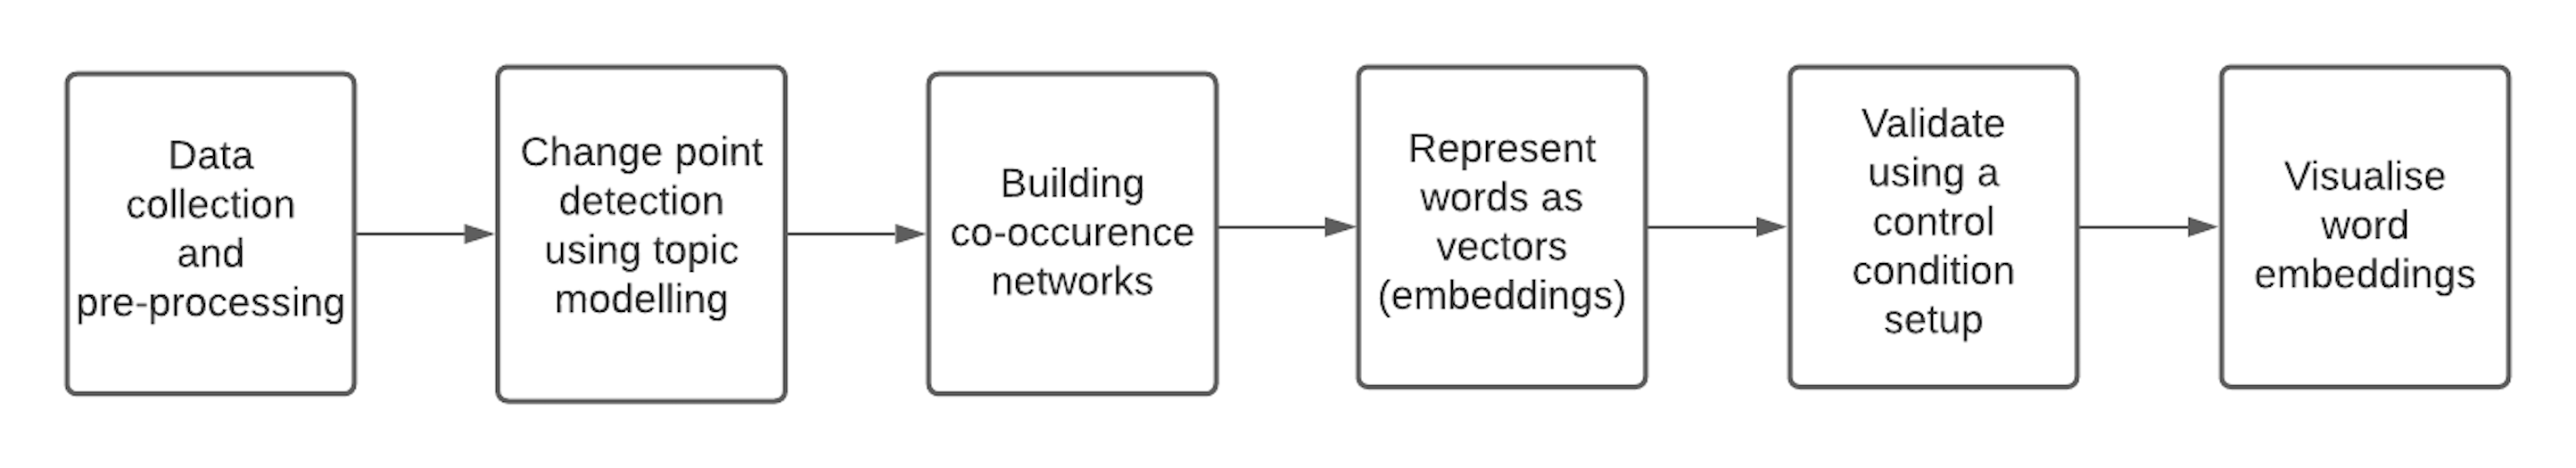
\includegraphics[width=\textwidth]{figures/MAHANTY_Methodology.png}
\caption{Methodology}\label{ch03:fig1}
\end{figure}

\subsection{Data collection and preprocessing}
As our first step towards our first research goal, we retrieved data in English from the Scopus\footnote{\url{https://www.scopus.com/home.uri}} database using the keyword ``circular economy'' from the period 2005--2019. The title, abstract, author keywords, index keywords and year of publication were retrieved and stored in a comma-separated values (CSV) format. We also collected full text articles from Elsevier in XML format. This corpus consisted of 3,300 articles. 
In order to fulfil our second goal of analysing the conceptual evolution of CE with respect to other concepts, we created a supplementary corpus of academic abstracts on 20 other concepts that have similar or overlapping conceptualisations with CE from the period 2005--2019. The related concepts are based on literature \citep{d2017green, geisendorf2018circular} and a Delphi study,\footnote{A Delphi study is a forecasting process framework based on the results of multiple rounds of questionnaires sent to a panel of experts. Several rounds of questionnaires are sent out to the group of experts, and the anonymous responses are aggregated and shared with the group after each round. We asked a question to the academic researchers about what other concepts they use in their research apart from ``circular economy'' and they provided other overlapping concepts which they tend to use in their research articles.} which we conducted with 66 academic researchers working on the CE concept. The 20 related concepts and their definitions are presented in Appendix~\ref{sec:05:appendix}. A total of 61,444 abstracts was included  in this supplementary corpus. In the preprocessing step we removed all instances of punctuation from the data, then the data was lower-cased and tokenised.

\subsection{Change point detection}
\label{ch03:changepointdetection}
There has been a divergent policy articulation of the CE concept differentiating between its Chinese and European framings \citep{mcdowall2017circular}. Based on such insights from the literature we  hypothesise that there was a change in the concept of CE within the period of study i.e., 2005--2019. We seek to determine whether the concept changed significantly, and if yes, to estimate the point in time when this happened. The formulation of the task as change point detection is appropriate because even if a word might change its meaning (usage) only gradually over time, we can expect that there will be  a time period when the new usage becomes much more dominant \citep{aminikhanghahi2017survey}. The identification of a change point is important because this will further form a basis for division of the corpus into ``epochs'' for further analysis. There have been various methods used for change point detection such as frequency analysis, syntactic analysis and distribution-based methods \citep{kulkarni2015statistically}. In this study we implement a distribution-based method to identify a change point. 
Specifically, our methodology is underpinned by topic modelling, a statistical approach whereby non-exclusive groupings of words (i.e., topics) are automatically induced based on their distribution in a corpus \citep{nikolenko2017topic}. In topic modelling, every document (e.g., a journal article) is considered as consisting of a mixture of a number of topics, referred to as $k$. A well-known algorithm for topic modelling is Latent Dirichlet Allocation (LDA) \citep{blei2003latent}, which we applied over the entire corpus using the lda \citep{chang2011lda} and topic models \citep{hornik2011topicmodels} R packages. For each document $d$ in the corpus, LDA computes the probability that $d$ belongs to topic $t$, where $t$ is any of the $k$ topics automatically identified. The probabilities for each topic are then summed for each year based on the year of publication of each document. The sums are then visualised graphically in a stacked plot to assess the trend in the topics over the years. The determination of the number of topics and validation of the results is based on our previous work \citep{mahanty2019studying}. We use the change point as reference to slice the corpus into two subsets with each subset belonging to before and after the change point. We refer to the documents in the period before the change point as the early dataset and those published in and after it as the contemporary dataset.

Once we have the proportion of the topics for each year from 2005--2019 we find the mean topic proportion for each topic in the two subsets of the corpus. Then, we run a paired $t$-test overall for all the topics which further assesses if the point of change is statistically significant. 

\subsection{Building co-occurrence networks}
\begin{sloppypar}
Co-occurrence vectors are employed in various ways to detect word level changes such as in context vectors, pointwise mutual information, temporal random indexing, or entropy in word level change detection \citep{tahmasebi2018survey}. We develop co-occurrence networks based on the keywords associated with the documents. Visual keyword frequency data provides useful insights by revealing predominant trends in the keyword network of the analysed literature demonstrating a birds-eye view knowledge map \citep{li2019trends}.
In our study, nodes of the network correspond to the keywords (with a node for CE as the centroid), and edges indicate the co-occurrences; edge thickness represents the frequency of co-occurrence. A co-occurrence network was generated using the bibliometrix package\footnote{\url{http://bibliometrix.org}, \citet{aria2017bibliometrix}.} in R, for each of the epochs that was identified in the previous step. The development of the co-occurrence network is the first step to detecting the nature of changes in the concept diachronically in the two epochs. 
While keyword co-occurrence networks provide simple and high level information of a field, such networks are limited in their capacity because they only focus on high frequency words. Inclusion of words with lower frequencies will limit the interpretability of the network structure.
\end{sloppypar}

\subsection{Training word embedding model}
Word embeddings map high-dimension word vectors (usually produced using simple one-hot encoding representations) to low-dimension vectors to obtain global semantics \citep{tang2018state}. Word embedding techniques that rely on the local context of the target words include Word2vec \citep{mikolov2013efficient} and Glove \citep{pennington-etal-2014-glove}. We trained two word embedding models using Word2Vec, one for each of the early and contemporary datasets. For this, we made use of the gensim package,\footnote{\url{https://radimrehurek.com/gensim/ models/word2vec.html}, \citet{rehurek_lrec}.} with a context window of four tokens and vector dimensionality of size 300 in line with the settings that have been used in previous work \citep{hamilton-etal-2016-diachronic}. The word embedding vectors were trained on each epoch and then aligned using orthogonal Procrustes transformation \citep{schonemann1966generalized} which has been applied to detect semantic change between different time periods \citep{hamilton-etal-2016-diachronic,dubossarsky-etal-2017-outta, abercrombie2019semantic}. We then compared word embedding vectors for the word of interest ``circular economy'' across the different time windows by calculating the cosine similarity between their embedding vectors calculated based on the two different periods. A lower cosine similarity between vectors is indicative of higher difference in the meaning, usage and context of a term.
\subsection{Validation of word embedding model using a control condition setup}
We test the results obtained from word embeddings based on a control condition setup, given that \citet{dubossarsky-etal-2017-outta} identified some studies where semantic changes are largely spurious results of the word representation models on which they are based. Until we have sufficient knowledge about the interpretation of conceptual changes, inferences need to be drawn with care and verified through multiple methods \citep{sommerauer2019conceptual}. Thus, we use a control condition setup to validate the results drawn from the word embeddings. 

Complementary to the genuine condition, a control condition is created where no change of meaning is expected. The underlying assumption is always that within the same dataset, the ``circular economy'' concept did not change its meaning. Again, unlike in the genuine condition, any changes that are observed can be attributed only to ``noise'' that stems from random sampling, rather than any real change in the usage or context of the concept. Therefore, any observed change in a word's meaning in the control condition can only stem from random ``noise'', while changes in meaning in the genuine condition are attributed to ``real'' semantic change in addition to ``noise''. In order to create a control condition we randomly sample the early dataset into two subsets (referred to as subsets A and B) and similarly created two random samples from the contemporary dataset  (subsets X and Y). We then compute the mean cosine similarities between the word vectors of A and B and those of X and Y. 

\subsection{Comparison of CE with respect to other concepts}
Word embedding models are known to successfully capture complex relationships between concepts, as manifested in the well-known word analogies task \citep{mikolov2013-distributed}, where a model aims to ``solve'' equations of the form ``A is to B is as C is to what?'' A classical example that is often used in distributional models is capturing the relation between \emph{man} and \emph{woman} is same as \emph{king} and \emph{queen} (by adding and subtracting the corresponding word vectors). Thus, it is a natural development to investigate whether changes in semantic relationships across time can also be traced by looking at the diachronic development of different distributional models \citep{kutuzov-etal-2018-diachronic}. Drawing from this idea we proceed with detecting changes in the CE concept in relation to other concepts. 
We construct a database of academic abstracts on 20 concepts that have similar or overlapping conceptualisations with CE from the period 2005--2019. Firstly one with all abstracts from the Scopus database using each of the 20 concepts and CE abstracts from the early period and second with all abstracts on the 20 concepts and CE abstracts from the contemporary period (identification of period based on Section~\ref{ch03:changepointdetection}).  We again align the two models using orthogonal Procrustes and calculate the cosine distance of CE with the 20 other concepts in the early and contemporary period. 

\section{Experiments}\label{ch03:experiments}
In this section we present the results that we obtained following the methodology.

\subsection{Change point detection}
We summarise the results from the topic modelling in Figure~\ref{ch03:fig2}. Based on the results of topic modelling \citep{mahanty2019studying} we identify two structurally different periods in the literature on CE. A structural change in the relative proportion of the identified topics was visually detected in the year 2015. In order to identify if the change in the year 2015 was significant we run a paired $t$-test based on the mean topic proportions in the early and the contemporary dataset. In the paired $t$-test the null hypothesis is that the mean difference between the two sets of observations is 0. A statistically significant $p$-value at 0.042 leads us to reject the null hypothesis and is supportive of our decision to divide the corpus into two epochs.\largerpage[2]

\begin{figure}[H]
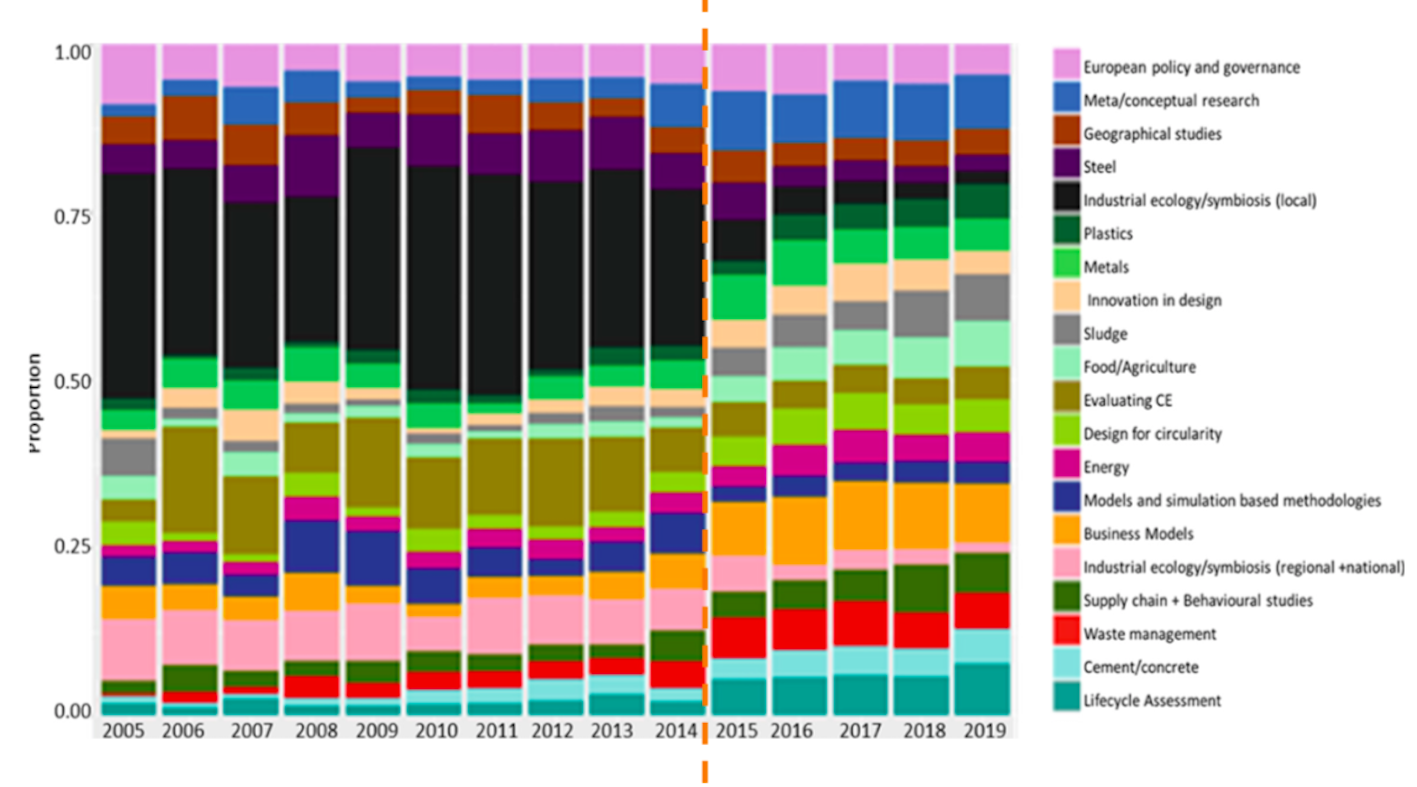
\includegraphics[width=\textwidth]{figures/MAHANTY_Change detection.png}
\caption{Visual representation of topic modelling and point of change} \label{ch03:fig2}
\end{figure}\clearpage
\largerpage[2]
\vfill
\begin{figure}[H]
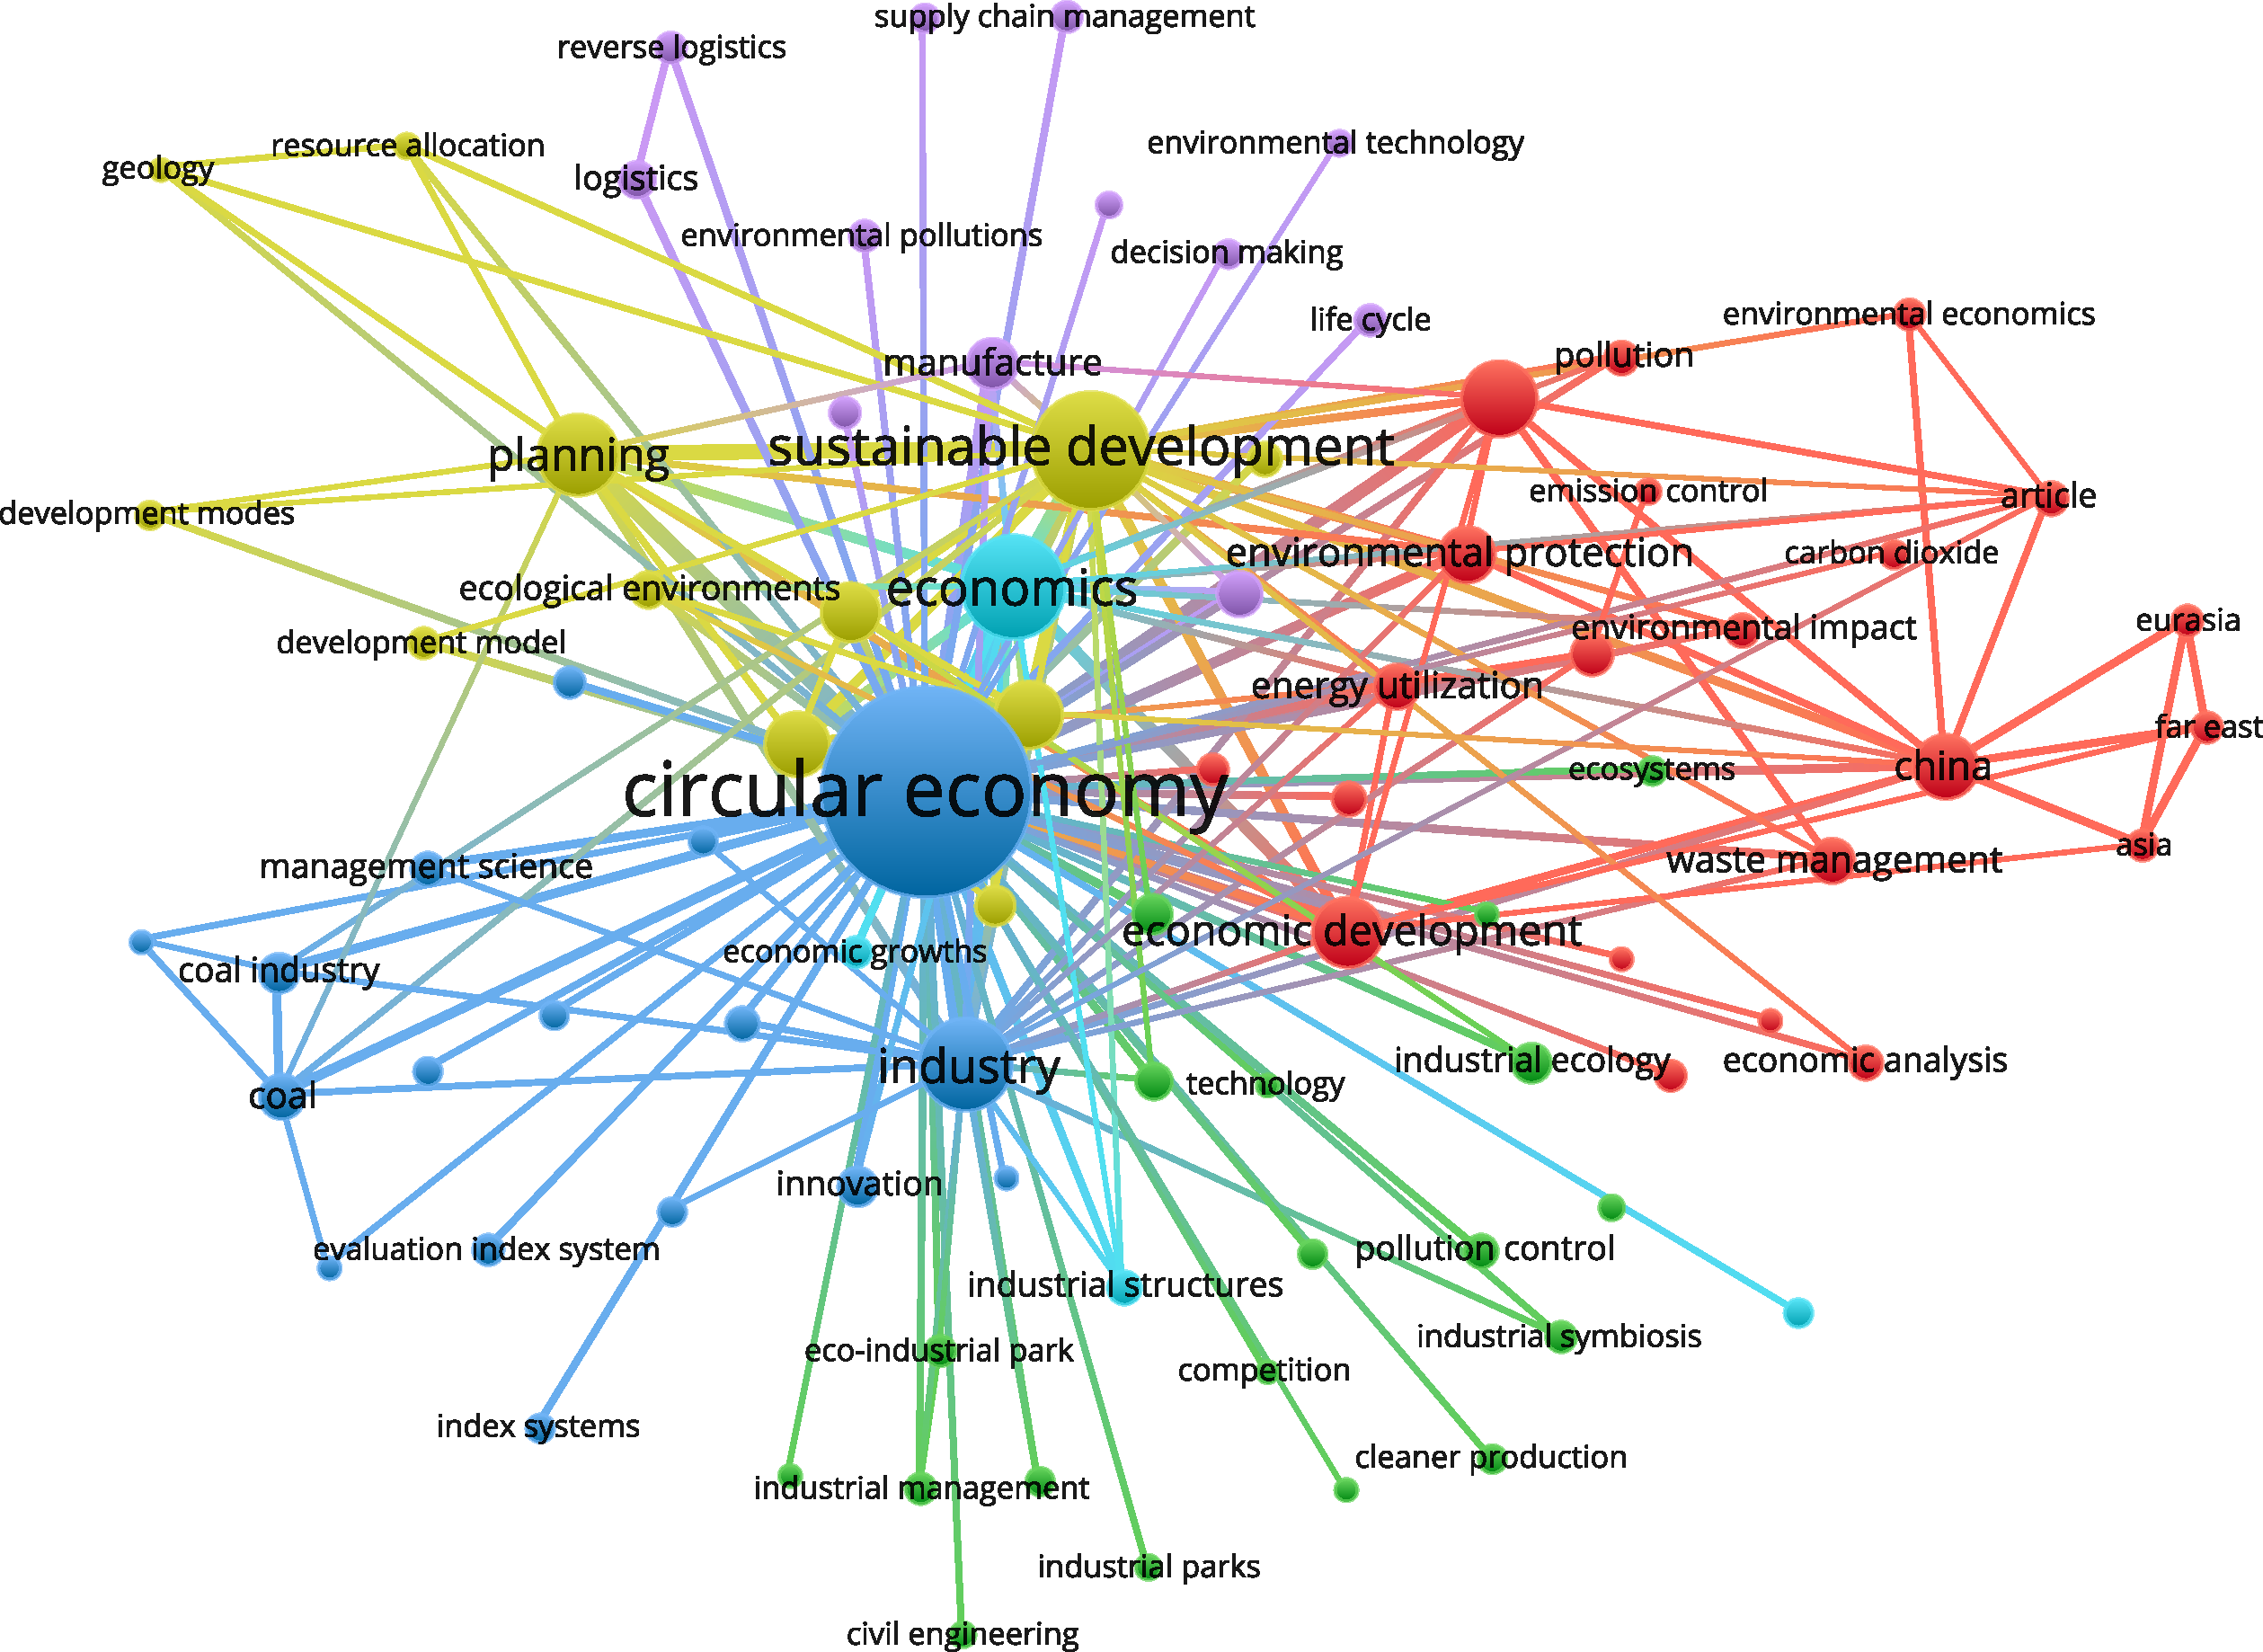
\includegraphics[width=.9\textwidth]{figures/MAHANTY_Co-occurrence1.pdf}
\caption{Co-occurrence network of the early dataset (2005--2014)}\label{ch03:fig3}
\end{figure}
\vfill
\begin{figure}[H]
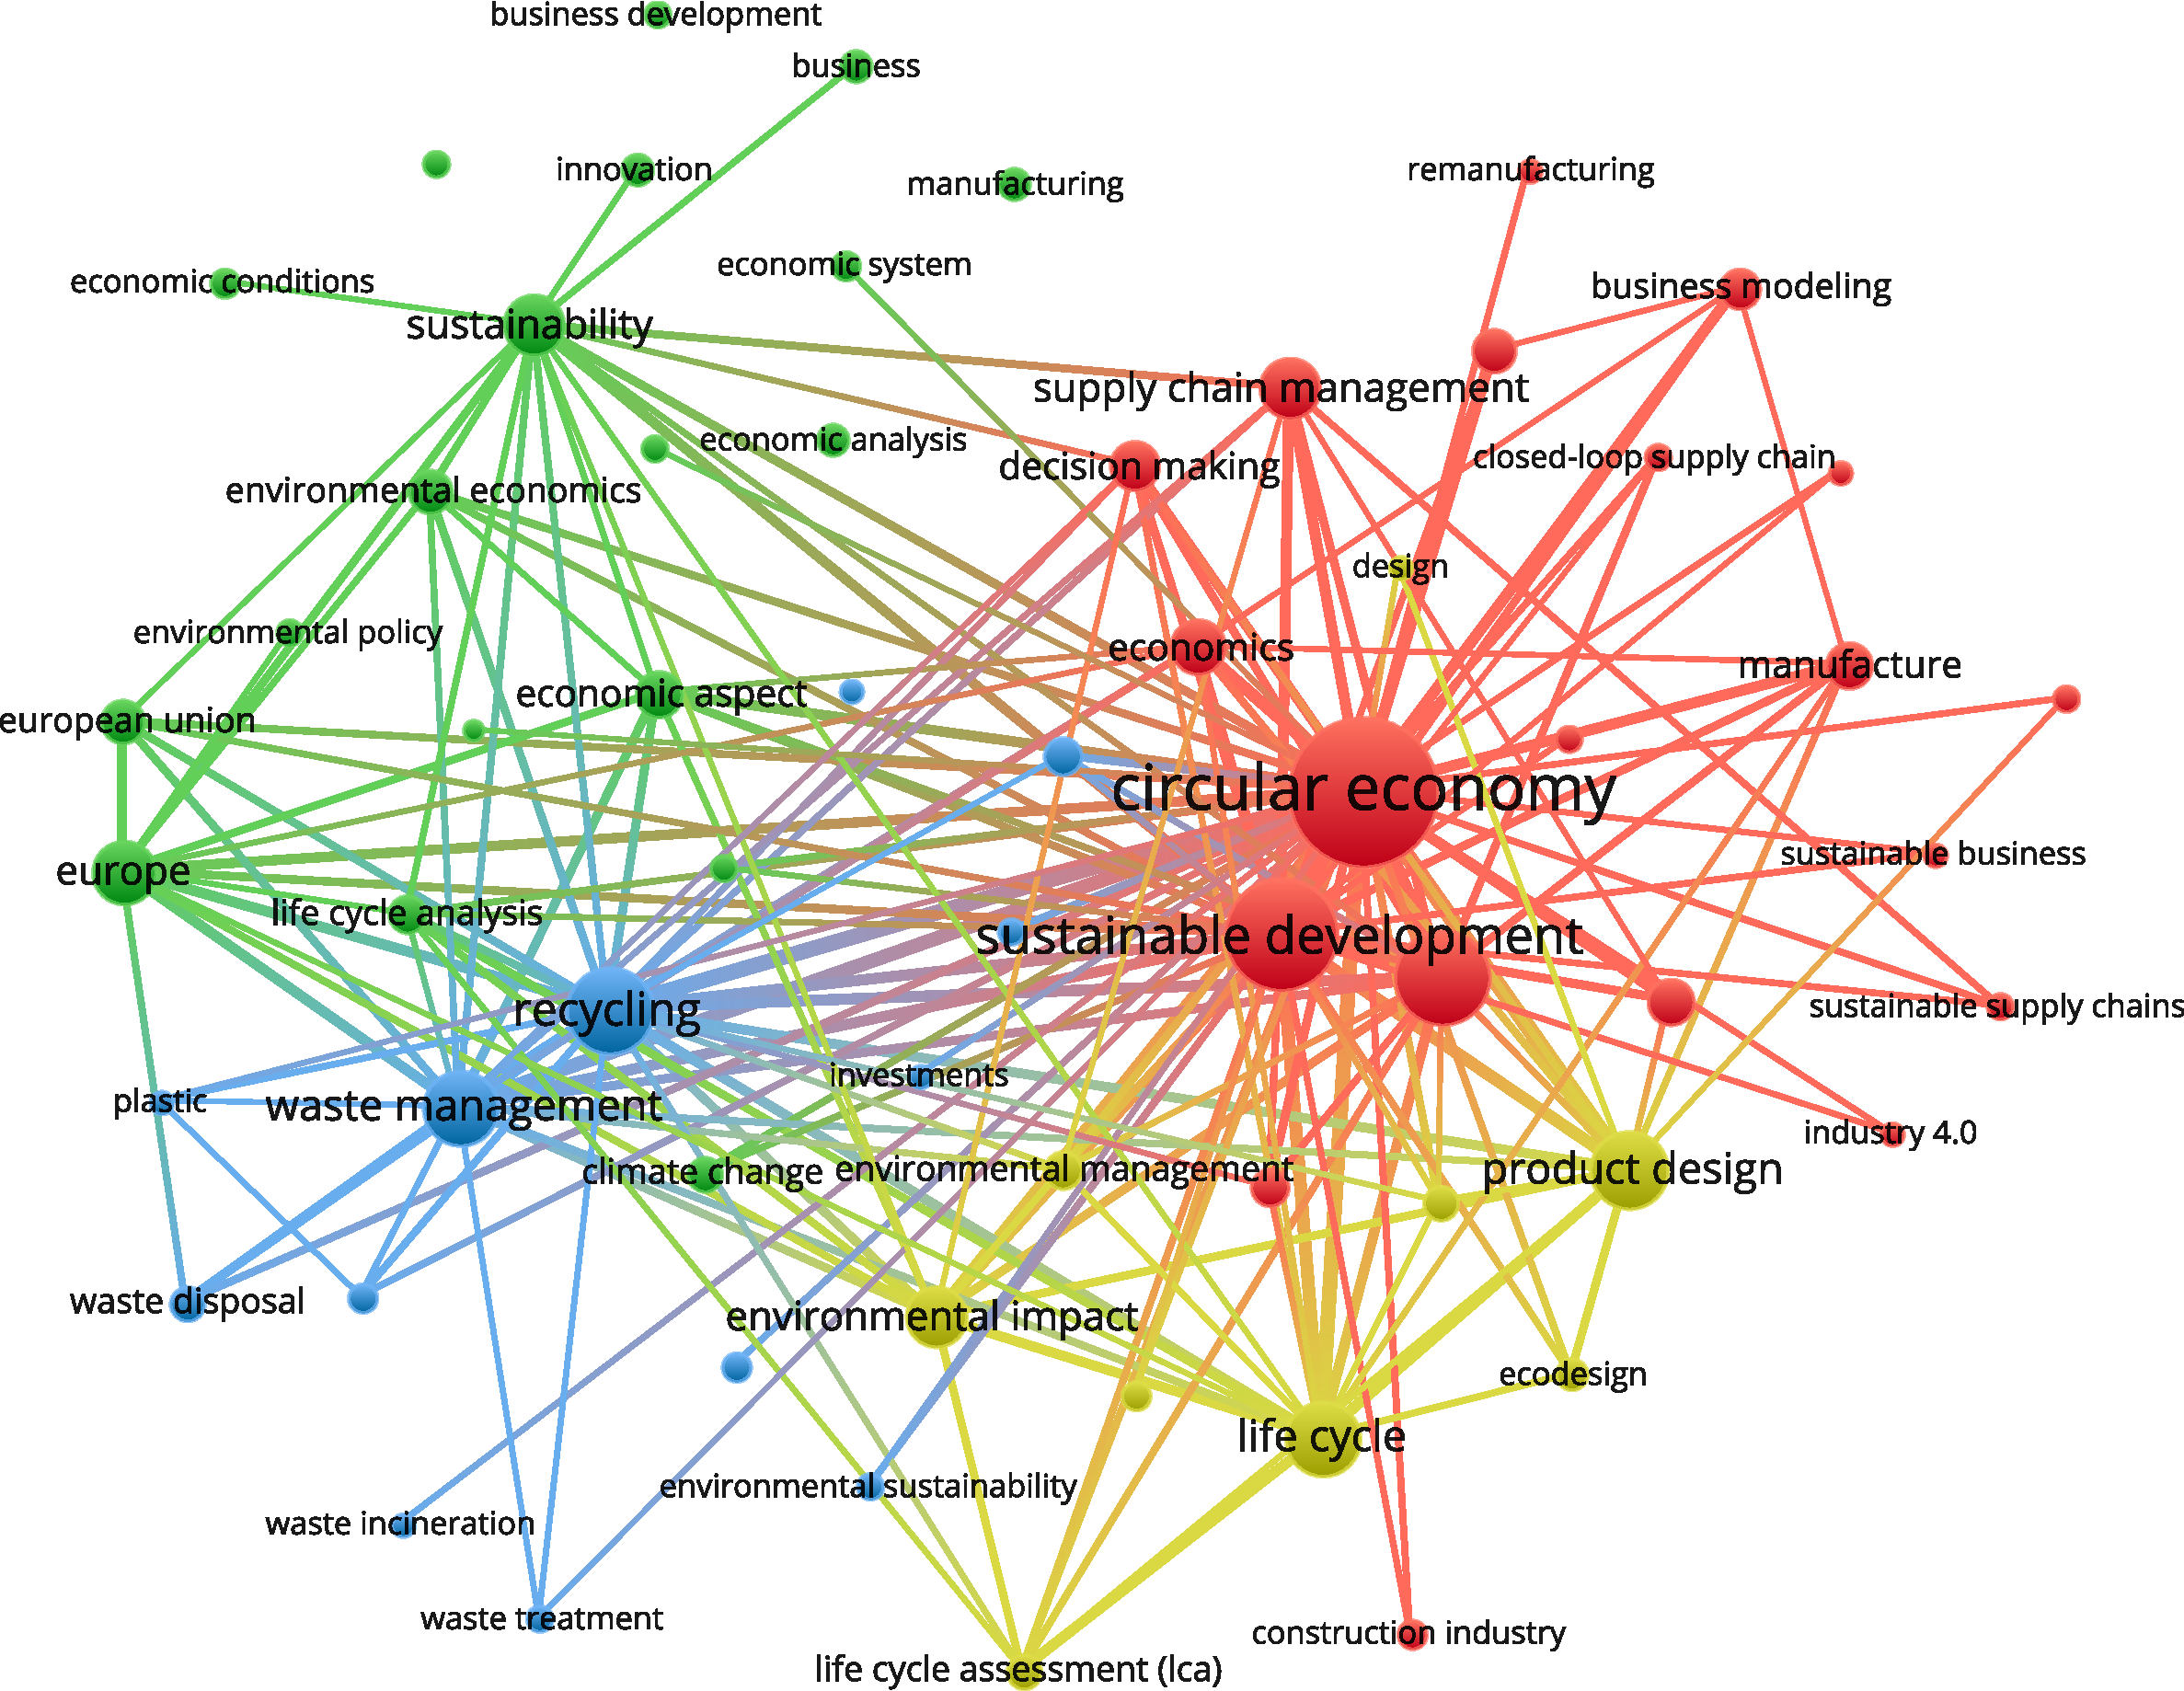
\includegraphics[width=.9\textwidth]{figures/MAHANTY_Co-occurrence2.pdf}
\caption{Co-occurrence network of the contemporary dataset (2015--2019)}\label{ch03:fig4}
\end{figure}
\vfill\clearpage

\subsection{Co-occurrence networks}
On developing keyword co-occurrence networks for each of the two datasets, i.e., early and contemporary, we observed certain differences between the structures.
Contemporary CE literature was found to be more strongly linked to \emph{business models}, \emph{supply chain}, and \emph{product design}. Meanwhile the focus of early CE literature was more on \emph{ecology}, \emph{industrial economics} and \emph{environmental management}. These observations confirm that the concept of CE has undergone some change over the years that are reflected by a shift in focus in the context of its application. We note that despite this expansion, the core meaning of the concept has not changed over time (as evidenced by the nodes that are common between the two networks, for example, \emph{sustainable development}, \emph{waste management}, \emph{recycling}).

\subsection{Word embeddings}
After training word embeddings on each of the two datasets and aligning them using orthogonal Procrustes transformation we examined the nearest neighbours of CE (i.e., words with highest similarity to CE). We see a shift from the environmental and industrial focus to a perspective which integrates innovation with a business focus and also incorporates the social dimension of CE. The results from the word embeddings are in agreement with the results from the co-occurrence networks. The early literature primarily addressed macro-level themes in the context of environmental management and industries while the contemporary literature focuses on more micro-level interventions like business models, product design and supply chain. However, words such as \emph{sustainability} and \emph{sustainable development} consistently dominated the literature in both of the time periods, both of them being key to  the conceptualisation of CE. The mean cosine similarity between word embedding vectors across the two time frames, i.e., early and contemporary, is only 0.195 which is quite low; this is not surprising, considering the extent of shift in the context of CE over time. We visualise the results from the word embeddings on a distributional space (Figure~\ref{ch03:fig5}) using t-sne \citep{maaten2008visualizing}
which visualises high-dimensional data by giving each datapoint a location in a two dimensional map. 
\begin{figure}
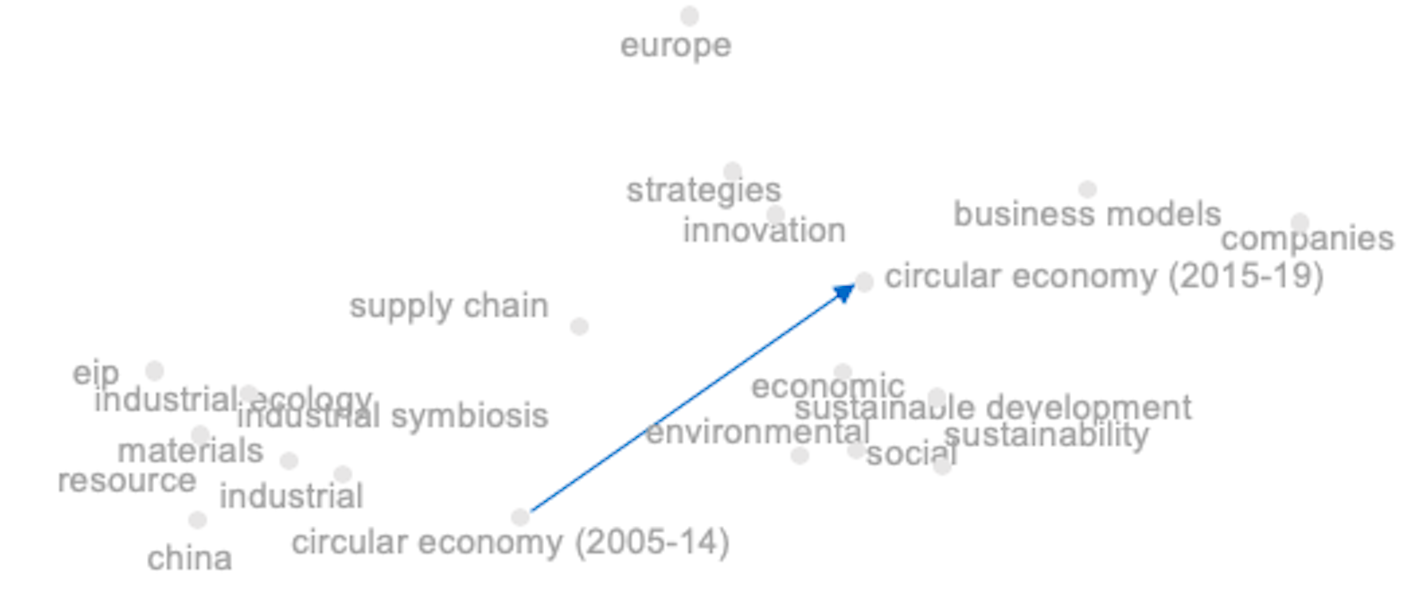
\includegraphics[width=\textwidth]{figures/MAHANTY_tsne1.png}
\caption{t-sne visualisation of CE based on the vectors in the early and contemporary period }\label{ch03:fig5}
\end{figure}

\subsection{Validation of results using a control condition setup}\largerpage[-1]
We observe the mean cosine similarity between the early and contemporary datasets is only 0.195. By using a control condition setup and creation of random subsets within the early and the contemporary period we find that the cosine similarity between the subsets drawn from the same time period was quite high, i.e., 0.62 and 0.743, for the early and the contemporary datasets, respectively. Thus, the low mean cosine similarity between early and contemporary datasets indeed indicates a change. 

\subsection{Comparison of CE with its overall semantic field}\largerpage[-2]
We compare CE with the overall semantic field and assess the relationships with the 20 concepts. In Figure~\ref{ch03:fig6} we present the semantic field in a distributional space using t-sne \citep{maaten2008visualizing}. This is based on training word embeddings on a corpus of journal abstracts on the 20 concepts and CE. The total corpus consists of 61,444 abstracts. The individual dots represent the collocational words corresponding to each concept. The solid circles denote positions in the distributional space which are characterised by the unique contextualisation of the concepts whereas the dotted circle represents a space which constitutes an overlapping context between the concepts and depicts inter-relationships that exist between these concepts. It is interesting to note here that the ``circular economy'' concept seems to have an overlapping conceptualisation with most concepts. The inter-related nature of the semantic field also points towards the fact that these concepts cannot be studied or analysed in silos and researchers in these areas need to have a holistic knowledge of the associated concepts. For further analysis to detect any shift in the meaning of CE across the two time periods we divide the corpus into two parts as we did before and compute the cosine similarities between ``circular economy'' and each of the other concepts in the early and the contemporary period. The similarity between CE and each of the other concepts is mapped in Figure~\ref{ch03:fig7}. We notice a shift in the CE concept with respect to the other concepts. Earlier the CE concept was more closely linked to ``eco-civilisation'' and ``low-carbon economy'' while in recent times it has a closer link to ``sharing economy'', ``natural capital'', and ``zero waste''.
\begin{figure}
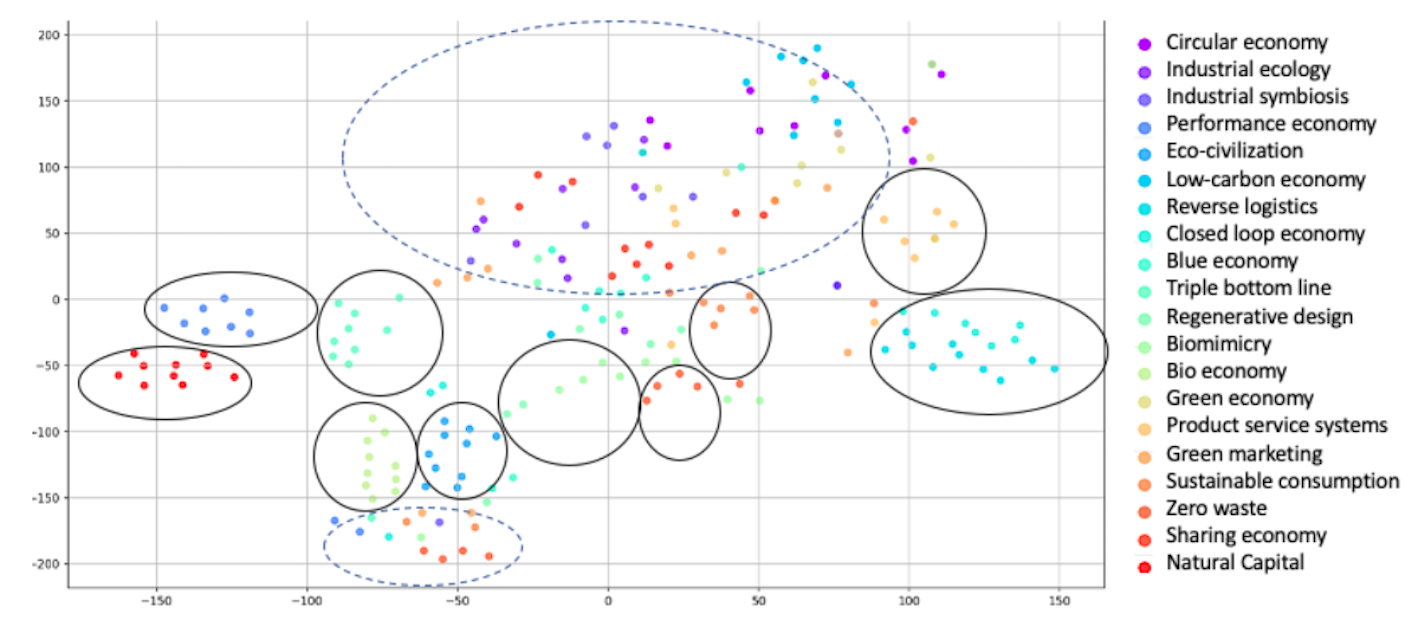
\includegraphics[width=\textwidth]{figures/MAHANTY_tsne2.png}
\caption{t-sne visualisation of the overall semantic field}\label{ch03:fig6}
\end{figure}

\begin{figure}
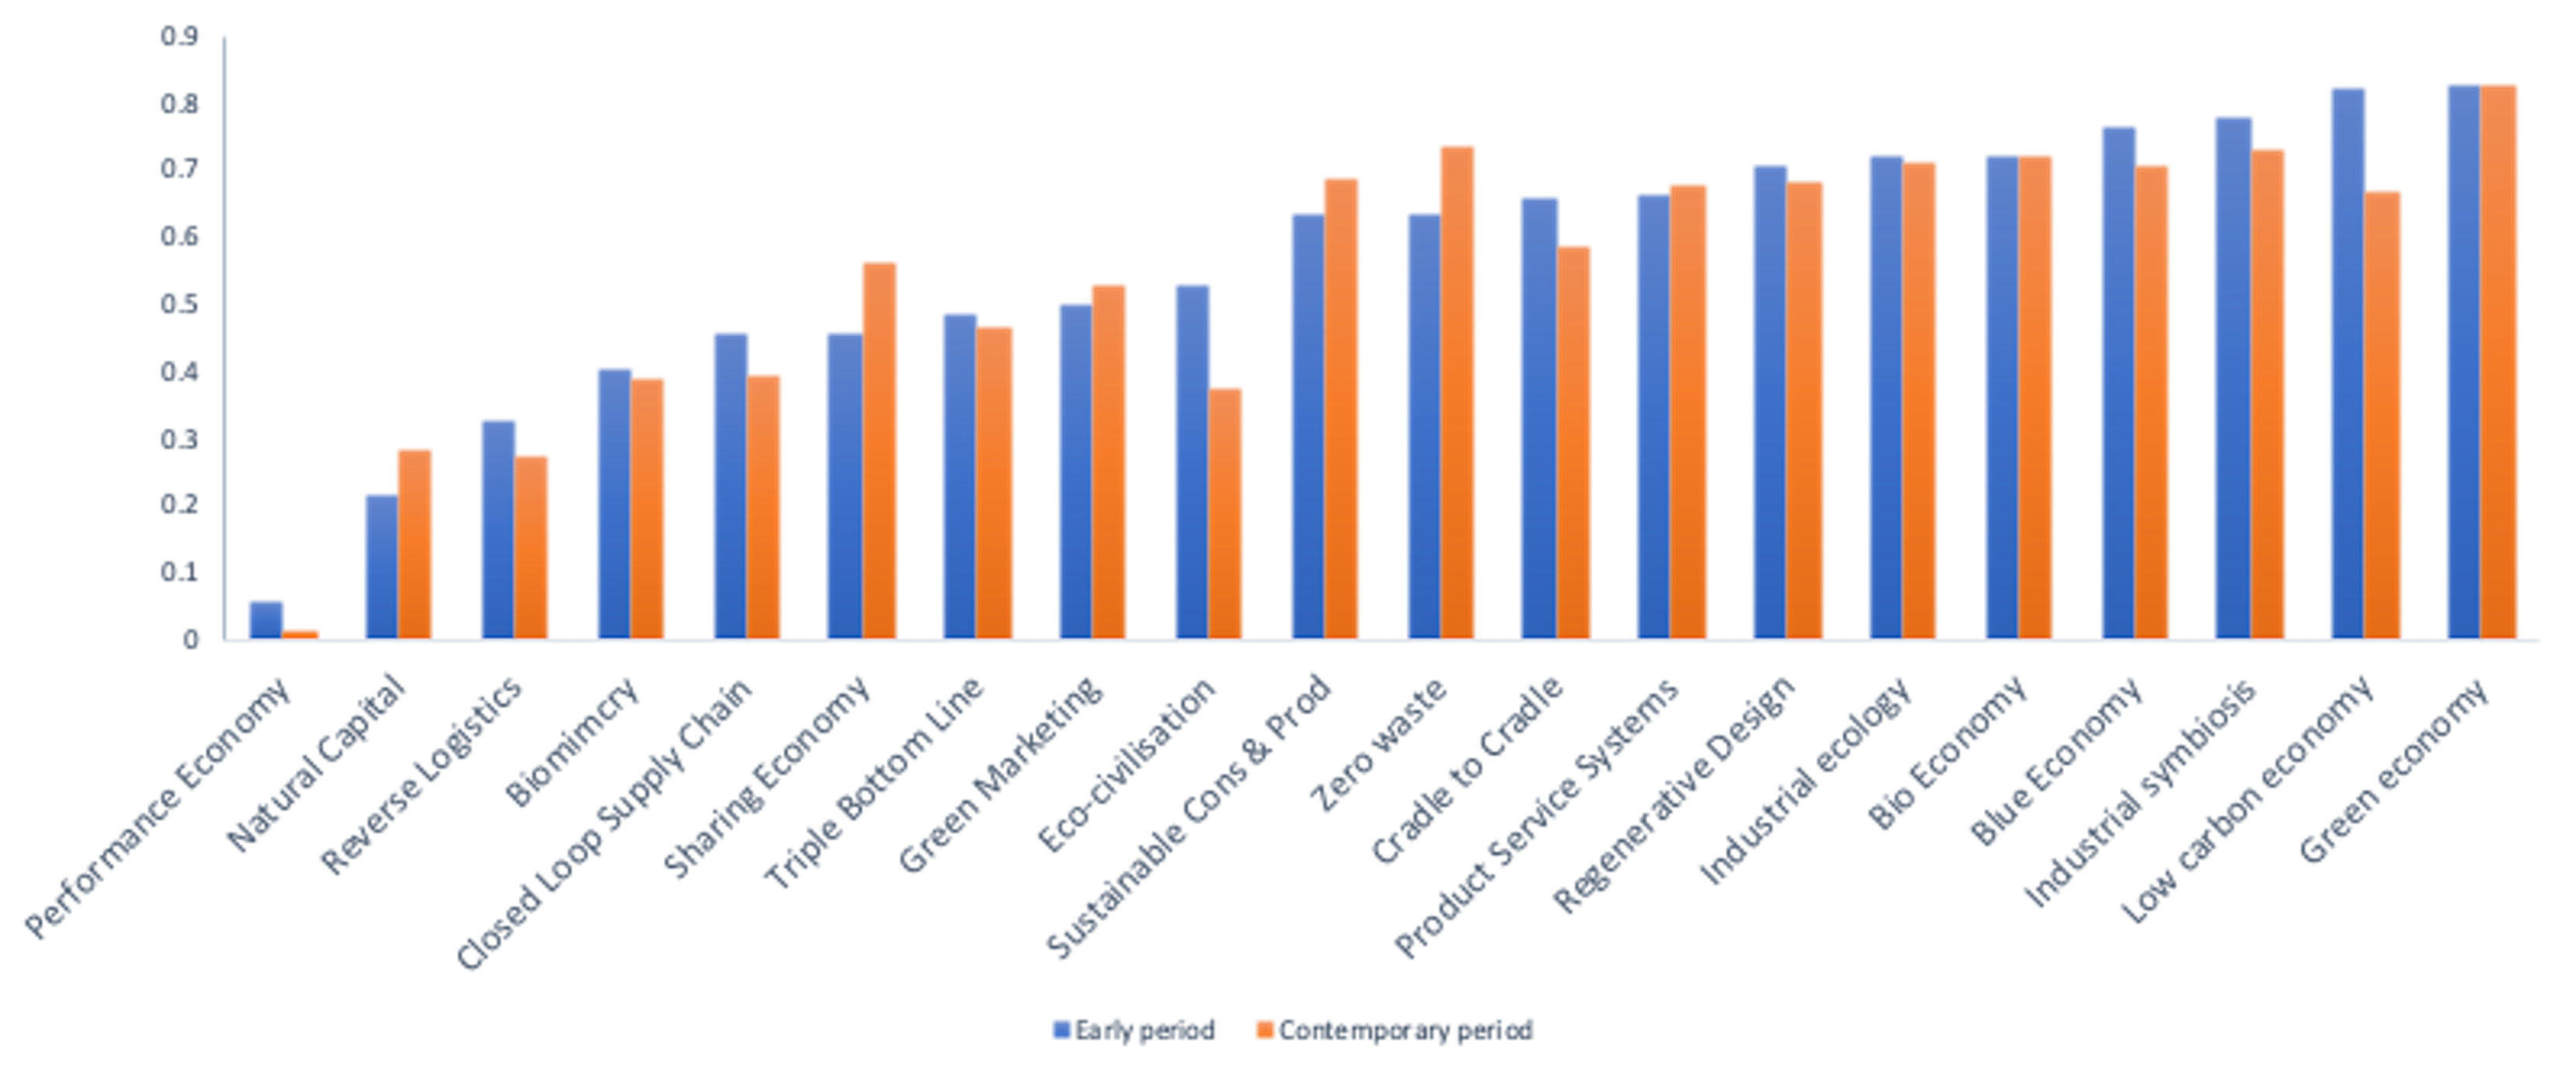
\includegraphics[width=\textwidth]{figures/MAHANTY_Cosine similarities.png}
\caption{Cosine similarities of CE with other concepts in each of the two datasets}\label{ch03:fig7}
\end{figure}

\section{Discussion and conclusion}\label{ch03:discussion}
In this chapter we presented a computational approach for analysing semantic change, which is underpinned by the automated discovery of topics within a corpus of 3,300 CE academic articles in English subdivided according to their year of publication. Applying an unsupervised topic modelling method based on Latent Dirichlet Allocation (LDA) on the entire corpus, a set of topics was identified for each of the years from 2005 to 2019. A significant structural change in the relative proportion of the identified topics was detected in the year 2015. Based on this observation the corpus was divided into two broad sets, i.e., 2005--2014 (early dataset) and 2015--2019 (contemporary dataset). 

To fulfill our first research objective and to detect changes in the CE concept, we compared the CE literature across these two time periods by applying on each of the data-sets two approaches -- building of co-occurrence networks and training of word embeddings using ``circular economy'' as the primary term of interest. We then aligned the word embeddings using orthogonal Procrustes and analysed the nearest neighbours of CE and their cosine distances. In order to fulfill our second research objective to detect changes in the CE concept in relation to other concepts, we created a database of academic abstracts on 20 concepts that have similar or overlapping conceptualisations with CE from the period 2005--2019. The related concepts are based on literature and a Delphi study which we conducted with 66 academic researchers working on the CE concept. We created two datasets, firstly one with all abstracts on the 20 concepts and CE abstracts from the early period (30,762 abstracts) and second with all abstracts on the 20 concepts and CE abstracts from the contemporary period (30,682 abstracts). We again aligned the two models using orthogonal Procrustes and calculated the cosine distance of CE with the 20 other concepts in the early and contemporary period. 
We found that the results from co-occurrence networks and word embeddings are consistent with each other, both showing that the concept of ``circular economy'' has undergone semantic change. Semantic change could mean two things: either the evolution of the word usage to the point that the modern meaning is radically different or semantic change by words acquiring additional meanings rather than original meanings being outdated or being replaced. In this study we have observed the latter in the context of CE. 

Specifically, our results provide computational evidence -- based on three different approaches -- for three main findings. Firstly, the core meaning of the concept has remained the same; this is evidenced by some common nodes in the results from the co-occurrence networks and nearest neighbours of CE based on word embeddings, such as ``sustainable development'', ``waste management'' and ``recycling''. Secondly, the concept has undergone some significant expansion, where the contemporary literature on CE was more strongly linked to ``business models'', ``supply chain'' and ``product design''. In contrast, the focus of early literature was more on ``ecology'', ``industrial economics'' and ``environmental management''. Thirdly, there is a slight shift in the closeness of meaning between CE and the other concepts across the two time periods. Earlier the CE concept was more closely linked to ``eco-civilisation'' and ``low-carbon economy'' while in recent times it has a closer link to ``sharing economy'', ``natural capital'', and ``zero waste''. The results are aligned with the history of CE where the early dataset relates to its antecedent concepts such as industrial ecology while the contemporary dataset is related to micro-level interventions for sustainable development. A further detailed analysis of the evolution of the CE concept and its relation to other concepts is beyond the scope of this paper.

From a methodological perspective, this approach could be used in assessing the evolution of concepts in academic discourse which is characterised by a vast corpus. In previous works of detecting concept change using computational methods, there have been no studies which focussed on evolution of concepts in the process of scientific knowledge production. This allows researchers to analyse large amounts of data which cannot be analysed using manual inspection. The computational methods discussed through the case study of ``circular economy'' could be broadly applied across disciplines. It will allow researchers to get an overview of the concept. Secondly it enables researchers to observe any high-level changes in a concept and can identify  certain research directions to pursue especially in the case of vast and expanding fields. We believe that this study will be helpful for both researchers already working on related topics as well as those new to the field, for example PhD candidates who wish to quickly grasp the recent advances and history of a field and pinpoint promising research opportunities and directions. Thirdly, more often than not there are multiple concepts that exist in a particular domain and a high level analysis of the overall semantic field provides the researcher with a fair understanding of the inter-relationships between the concepts. Along with that, from a conceptual perspective an evolutionary analysis could also aid in verifying hypotheses posited by linguists, anthropologists or other researchers in a field.

\appendixsection{Related concepts and definitions}\label{sec:05:appendix}

\begin{description}[font=\normalfont,noitemsep]\sloppy
\item[``industrial ecology'':] Systems view which seeks to optimise the total materials cycle, from virgin materials, to finished material, to component, to product, to obsolete product, \& to ultimate disposal.
\item[``industrial symbiosis'':] Engaging traditionally separate industries in a collective approach to competitive advantage involving physical exchange of materials, energy, water, and by-products.
\item[``performance economy'':] Represents a full shift to servitization, with revenue obtained from providing services rather than selling goods.
\item[``eco-civilisation'':] Inclusion of environmental protection in the nation's economic, social, cultural, \& political systems.
\item[``reverse logistics'':] Process in which a manufacturer systematically accepts previously shipped products or parts from the point for consumption for possible recycling, re-manufacturing, or disposal.
\item[``cradle to cradle'':] Minimizing environmental damage through sustainable production, distribution, disposal practices, \& socially responsible products.
\item[``blue economy'':] Optimization of natural marine resources within ecological limits, \& the decoupling of environment and economy.
\item[``triple bottom line'':] An accounting framework that incorporates three performance dimensions: social, environmental \& financial.
\item[``regenerative design'':] Principle that calls for products or services to contribute to systems that renew or replenish themselves.
\item[``biomimmicry'':] Studies natures best ideas and then imitates the designs \& process to solve human problems.
\item[``bio economy'':] Includes all economic activities that are linked to the development \& the use of biological products and processes.
\item[``green economy'':] System aimed at improved ``well-being \& social equity, while significantly reducing environmental risks \& ecological scarcities''.
\item[``product service systems'':] Combination of products \& services in a system that provides functionality for consumers \& reduces environmental impact.
\item[``green marketing'':] Activities designed to generate and facilitate exchanges intended to satisfy human needs or wants, such needs and wants are satisfied without environmental impact.
\item[``sustainable consumption and production'':] Use of services \& products, which fulfill basic needs, bring about a better quality of life while minimizing natural resource use, toxic materials \& reduce emissions thereby not jeopardising future generations.
\item[``zero waste'':] An aspirational end point where all waste is reused or recycled as a resource without the need for any landfill or energy recovery.
\item[``sharing economy'':] Forms of exchange facilitated through online platforms, aimed at open access to under-utilised resources through what is termed ``sharing''.
\item[``natural capital'':] An approach for protecting the biosphere \& for improving profits and competitiveness that benefits the current and future generations.
\item[``low-carbon economy'':] Economy based on low energy consumption \& low pollution.
\item[``closed loop economy'':] Used synonymously with the ``circular economy''.
\end{description}

\section*{Acknowledgements}
The authors declare no conflict of interest. Sampriti Mahanty would like to thank Alliance Manchester Business School for supporting this research work.

\section*{Abbreviations}
\begin{tabularx}{\textwidth}{@{}lQ@{}}
ACL & Association for Computational Linguistics\\
ACM & Association for Computing Machinery\\
LDA & latent Dirichlet allocation\\
LSA & latent semantic analysis\\
OCR & Optical Character Recognition\\
XML & eXtensible Markup Language\\ 
\end{tabularx}

{\sloppy\printbibliography[heading=subbibliography,notkeyword=this]}
\end{document}
